%!TEX TS-program = pdflatex 
%
\documentclass[journal]{IEEEtran}
%\documentclass[journal]{IEEEtran}


% *** GRAPHICS RELATED PACKAGES ***
%
\ifCLASSINFOpdf
  % \usepackage[pdftex]{graphicx}
  % declare the path(s) where your graphic files are
  % \graphicspath{{../pdf/}{../jpeg/}}
  % and their extensions so you won't have to specify these with
  % every instance of \includegraphics
  % \DeclareGraphicsExtensions{.pdf,.jpeg,.png}
\else
  % or other class option (dvipsone, dvipdf, if not using dvips). graphicx
  % will default to the driver specified in the system graphics.cfg if no
  % driver is specified.
  % \usepackage[dvips]{graphicx}
  % declare the path(s) where your graphic files are
  % \graphicspath{{../eps/}}
  % and their extensions so you won't have to specify these with
  % every instance of \includegraphics
  % \DeclareGraphicsExtensions{.eps}
\fi



%\documentclass{sig-alternate1}
%\documentclass{acm_proc_article-sp}
\usepackage{algorithmic}
\usepackage{algorithm}
%\usepackage{subfigure}
%\usepackage{algorithm2e}
%\usepackage{graphicx}
\usepackage{epsfig}
\usepackage{cite}
%\usepackage{aspdac}
%\usepackage{threeparttable}
\usepackage {amsmath}
\usepackage {multirow}
\usepackage{amsfonts}
\usepackage{subcaption}
\usepackage{color}
\newtheorem{proposition}{Proposition}
\newtheorem{property}{Property}
\newtheorem{lemma}{Lemma}
\newtheorem{theorem}{Theorem}


% *** Do not adjust lengths that control margins, column widths, etc. ***
% *** Do not use packages that alter fonts (such as pslatex).         ***
% There should be no need to do such things with IEEEtran.cls V1.6 and later.
% (Unless specifically asked to do so by the journal or conference you plan
% to submit to, of course. )


% correct bad hyphenation here
\hyphenation{op-tical net-works semi-conduc-tor}


\begin{document}


%
% paper title
% can use linebreaks \\ within to get better formatting as desired

\title{Synthesis of Activation-Parallel Convolution Structures for Neuromorphic Architectures}

% make the title area
\maketitle
\begin{abstract}
Convolutional neural networks have demonstrated continued success in various visual recognition challenges. The convolutional layers are implemented in the activation-serial or fully parallel manner on neuromorphic computing systems. 
This paper presents an unrolling method that generates parallel structures for the convolutional layers depending on a required level of parallel processing. We analyze the resource requirements for the unrolling of the two-dimensional filters, and propose methods to deal with practical considerations such as stride, borders, and alignment. We apply the propose methods to practical convolutional neural networks including AlexNet and the generated structures are mapped onto a recent neuromorphic computing system. This demonstrates that the proposed methods can improve the performance or reduce the power consumption significantly even without area penalty. 
\end{abstract}

\begin{IEEEkeywords}
Deep Learning, Deep Neural Networks, Machine Learning, Neuromorphic Engineering
\end{IEEEkeywords}

\IEEEpeerreviewmaketitle



\section{Introduction}
Machine intelligence has been improving significantly with growing interest in deep learning. Among others, convolutional deep neural networks have demonstrated astonishing results in various visual recognition challenges, firing the enthusiasm for deep learning. The functionality of machines is now a match for that of humans in some specific applications~\cite{he2015deep}; however, the energy efficiency of today's computing platforms running deep learning models is not comparable to the human brain. For example, AlphaGo, the state-of-the-art Go program based on deep learning~\cite{silver2016mastering}, ran on a server cluster with 1920 CPUs and 120 GPUs possibly consuming several hundreds kilowatt, but the professional Go player, Sedol Lee, just consumed about 20W during the match of the century. 

The Von Neumann architecture employed in the conventional computing platforms uses a small number of complex, versatile processing elements (PEs) and tries to time-share them as much as possible. In order to improve the performance, we had increased the clock frequency using more pipelining stages but this backfired due to the unmanageable power dissipation~\cite{parkhurst2006single}. The paradigm has then shifted toward parallel processing, which now becomes the key to energy-efficient high-performance computing. For a higher level of parallel processing, we need to add more PEs on a silicon die. However, the silicon area is still expensive despite technology scaling, and some processors employ lightweight, less versatile PEs to increase the number of PEs. As the number of PEs increases, it becomes difficult to feed data to all the increased number of processing elements since the memory bandwidth is limited~\cite{burger1996memory} and scheduling becomes complex. In this situation, the number of cores is limited up to a few thousands. 

The extreme case of parallel processing is found in our brain. Our brain has about 100 billion neurons and over 100 trillion synapses. Synapses serve as memories as well as PEs. Neuromorphic engineering can be performed at many different levels and areas, and we can also mimic how so many PEs operate together. Recent neuromorphic architectures~\cite{merolla2014million,chung2015insight} equip with a huge number of low-cost processing elements and place the PEs and memories in proximity of each other. Then, the units and connections of a neural network are mapped into silicon neurons and synapses, respectively. This approach is very different from the traditional architecture, where the computational operations of the neural network are scheduled to PEs.

Convolution is one of the most fundamental operations in signal processing, and can be performed using digital hardware filters. Parallel processing is a common way to improve the throughput of the filters~\cite{parhi2007vlsi}. However, in practice, replicating hardware has not been very popular  because of the area overhead~\cite{tsao2012area}. For example, even a single multiplier takes up large area, and thus practical development and research have focused on time-sharing of multipliers. However, in neuromorphic architectures, tiny PEs such as memristors are available, and parallel processing is likely to become practical in the near future. 


Convolutional neural networks require a number of two-dimensional (2D) convolution operations. The 2D convolution with a $K\times K$ kernel for an image of $W\times H$ pixels can be reduced to a matrix-vector multiplication by unrolling the kernel. The matrix is roughly of the size $WH \times WH$ and approximately has $WHK^2$ non-zero elements. This matrix-vector multiplication is performed in the fully parallel manner in most neuromorphic architectures, and will require a huge number of synapses no matter how well the neuromorphic architectures handle the sparseness. The huge number of synapses still becomes a burden even if very low-cost PEs are available. In addition, we may also require a huge buffer for the entire image, and the entire inputs may not be available at the same time due to the limited I/O bandwidth. On the other hand, the 2D convolution can also be performed in a word-serial manner as 2D convolution hardware does. In this case, $K^2$ synapses are just needed, but it will take $W \times H$ time steps. Thus, a compromise between the two extremes is needed. There exists strong theoretic foundations for parallel one-dimensional FIR filters~\cite{parhi2007vlsi}, but there are fewer discussions for the two-dimensional case. Practical considerations such as border handling and stride in the parallel structures have little been studied in the literature.
 
In this paper, we propose an algorithm that synthesizes activation-parallel 2D filters for a required level of parallel processing and discuss the practical issues when it is applied to real-world convolutional neural networks. The major contributions of this paper can be summarized as follows:
\begin{itemize}
\item We analyze the resource requirements when 2D filters are unrolled.
\item We discuss how the practical issues such as stride, border handling, and alignment can be dealt with when we apply unrolling to the filters for convolutional neural networks.
\item We apply the propose method to a recent neuromorphic architecture and demonstrate that a neuromorphic computing system can really achieve a surprising throughput at ultra-low power.
\end{itemize} 

\section{Related Works} 
Parallel FIR filters have been extensively studied and it is well known that parallel processing structures can be automatically created by unrolling a given data flow graph~\cite{parhi2007vlsi}. Although the multidimensional synchronous dataflow (MDSDF) model has been proposed in~\cite{murthy2002multidimensional}, most studies in (multi-rate) signal processing deal with one-dimensional signals and there is little discussion about unrolling a MDSDF graph to our best knowledge. The parallel processing structures obtained by unrolling may be naive and the hardware cost increases linearly in the level of parallel processing. Fast FIR algorithm (FFA) based polyphase decomposition~\cite{tsao2012area} can reduce the hardware cost significantly, but it is effective when the tap size is large enough. Thus, its use may not be desirable for image filters, where kernel sizes are small usually.

Another common way to perform convolution in parallel is to divide a long signal into pieces and to convolve each in parallel. The convolution of each piece can also be performed via dot product in the time domain or via element-wise multiplication in the frequency domain using the discrete fourier transform (DFT). In order to obtain the linear convolution from the cyclic convolution of the frequency domain, the overlap-add method or the overlap-save method is commonly used. However, approaches of this type do not fit neuromorphic architectures well.

In this paper, we deal with parallel processing structures in two-dimensional cascaded filters and discuss all the practical considerations such as stride, border handling, and alignment. To our best knowledge, there is no well-established theory dealing with all these issues. 

\section{Preliminaries}

The neuron model commonly used in the machine learning community is called the perceptron. In this basic model, a neuron (a.k.a., unit) performs the computation
\begin{equation}
y = f(\sum_i^N{w_i x_i} + b)
\end{equation}
where $y$ is the \textit{activation} of the neuron, $N$ is the number of inputs, $x_i$ is the input activation, $w_i$ is the weight, $b$ is the bias, and $f$ is the activation function. A neural network is a composition of perceptrons. The neurons in the network are organized into layers depending on their levels in the network. The first layer is the input layer, the last layer is the output layer, and the other layers are the \textit{hidden layers}.
If a feedforward network has more than one hidden layer, we call it the \textit{deep} neural network.
\begin{figure}[h]
\centering
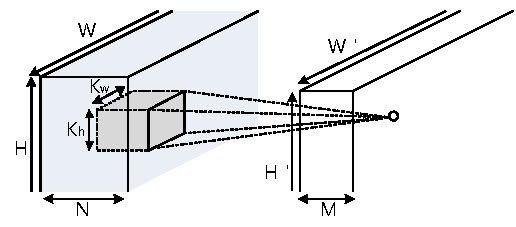
\includegraphics[width = 2.8in]{./FIGURES/fig1.pdf}\
\caption {Neurons in convolutional layers are arranged in a 3D space and have spatially local connections.} \label{cnn}
\end{figure}
Most common layer type is the fully connected layer where units between two adjacent layers are fully pairwise connected. Convolutional neural networks (CNNs) are multi-layer neural networks, and usually take an image as input. A CNN is made up of two main types of layers: convolutional layers and fully connected layers. 
Neurons in a convolutional layer are arranged in a three-dimensional space. 
The dimensions are height and width (the spatial dimensions), and depth. 
For example, input neurons activated by the pixels of each channel of an input image can be laid out according to 
vertical and horizontal positions of the pixels and the channels. 
Each convolutional layer of a CNN transforms the input activations, represented by a 3D volume, into a 3D output volume. Consider a convolutional layer that takes $N$ activation maps of size $H\times W$ and produces $M$ activation maps of size $H' \times W'$.
Each input activation map is convolved with a $K_h\times K_w$ kernel and the resulting maps are added up element-wise, yielding an output activation map. This is repeated $M$ times, leading to the $M$ activation maps. Thus, a convolutional layer requires $N\times M$ 2D convolutions. 
The convolutional layer is depicted in Figure~\ref{cnn}. The convolutional layer can be re-arranged in a one-dimensional space, forming a $WH \times W'H'$ layer, and this can be implemented in a neuromorphic architecture directly. However, it can also be converted into a time delay neural network (TDNN) that performs the same task in an activation-serial manner. The time delay neural network is equivalent to a dataflow graph representing a two-dimensional FIR filter. In the TDNN, an activation map is serialized into a stream of activations and it takes $H\times W$ time steps to complete the processing.  An example is shown in Figure~\ref{conv2tdnn}.
\begin{figure}[h]
\centering
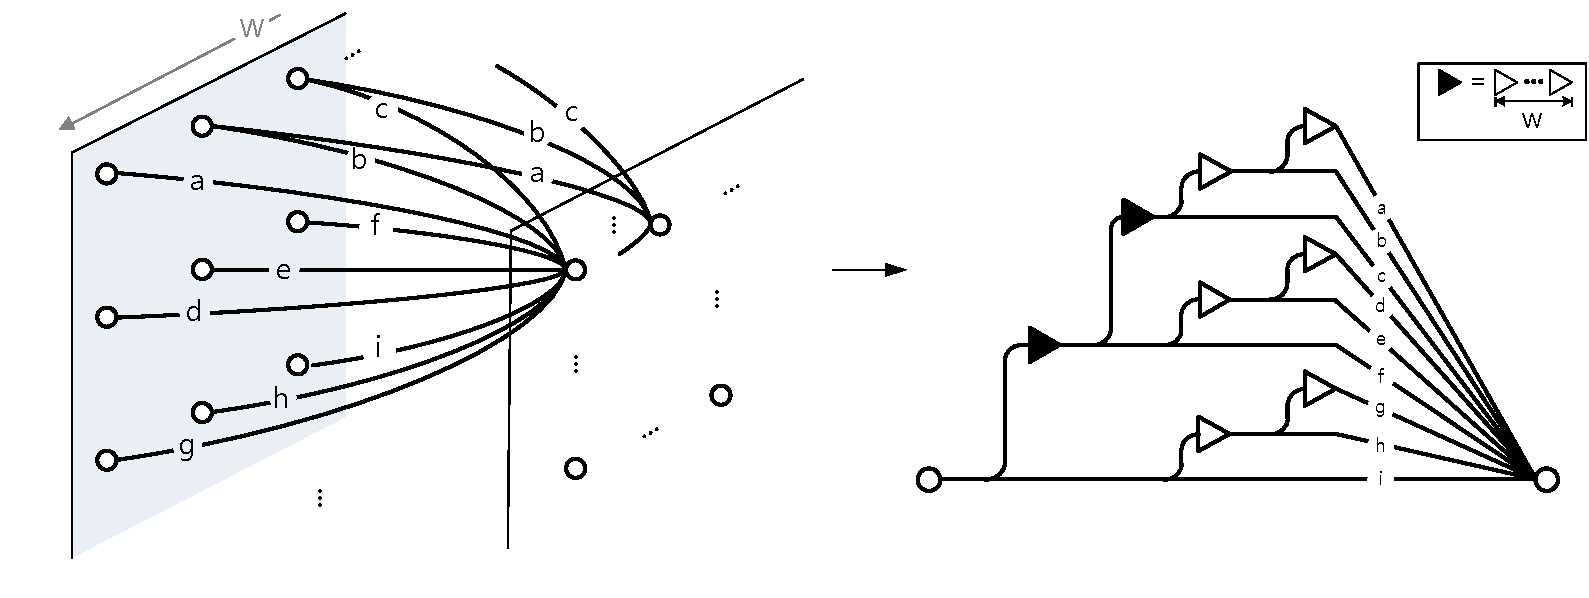
\includegraphics[width = 3.5in]{./FIGURES/fig2.pdf}
\caption {Convolutional layers are converted into a TDNN representing an activation-serial filter structure.} \label{conv2tdnn}
\end{figure}


%https://en.wikipedia.org/wiki/Overlap%E2%80%93add_method

\section{Activation-Parallel 2D Filters}
A 2D filter with a $K_h\times K_w$ kernel is applied to an input map of $H\times W$ activations. We parallelize the processing of the filter by unrolling so that it processes multiple activations in parallel. A parallel 2D filter processes a $L_h \times L_w$ \textit{block} of the input map in a time step. 
The level of the parallel processing is defined by the size of the block.

The filter is referred as the $L_h\times L_w$-parallel 2D filter. This parallel filter will generate a block of $L_h \times L_w$ activations in a time step.  %For typical convolution, $L'_h=L_h$ and $L'_w=L_w$. The case that they are different will be discussed in the next subsection. 
Each output activation is generated from a window of $K_h\times K_w$ input activations, which will be referred as the \textit{kernel window}.  All the output activations produced in a time step are generated from a window of $G_h \times G_w$ input activations, which will be referred as the \textit{group window}.  The group window is the smallest bounding box enclosing all of the kernel windows. Whenever we try to avoid repetition for each dimension, we use $K$, $L$, $G$, etc instead of $K_h$, $K_l$, $L_h$, $L_l$, $G_h$, etc. 
The size of a dimension of the group window is given by
\begin{equation}
	G = K + L-1.
\end{equation}
Figure~\ref{groupwindow} depicts the initial position of the group window. 
\begin{figure}[h]
\centering
\vspace{-0.2in}
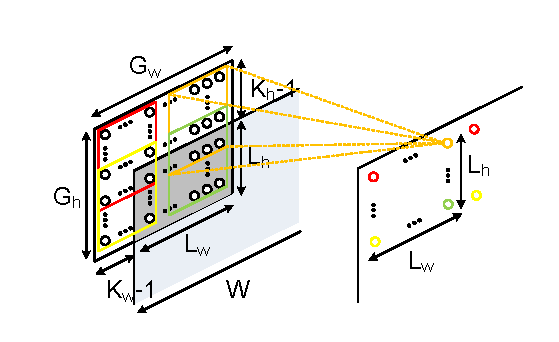
\includegraphics[width = 3in]{./FIGURES/fig3.pdf}
\vspace{-0.1in}
\caption {Activation-parallel filters take $L_h\times L_w$ activations in a time step and generates $L_h\times L_w$ activations at the same time. The other activations in the group window are obtained from delays, a special type of memories.} \label{groupwindow}
\end{figure} 
Filters are typically modeled as a dataflow graph in signal processing literature. However, we will model them as time delay neural networks since we will use them in neuromorphic architectures. Nonetheless, they can be converted to dataflow graphs very easily for use in other conventional systems. Delays are a type of short-term memory, and a chain of delays performs time-to-space conversion. It allows us to bring past activations in a stream of activations to the present. A \textit{line delay} is a chain of $W/L_w$ delays. We use a line delay (\textit{activation delay}) to bring a previous activation in the vertical (horizontal) direction to the current from an activation stream.   To generate the $L_h \times L_w$ activations in a time step, all the activations in the group window should be available at the same time, but we only have the $L_h\times L_w$ activations from the input neurons. The other activations in the group window become available by delays. Figure~\ref{tdnn} shows  a time delay neural network representing the parallel filter.
\begin{figure}[h]
\centering
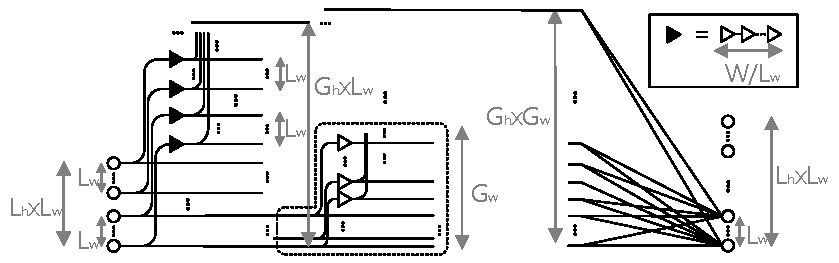
\includegraphics[width = 3.2in]{./FIGURES/fig4.pdf}
\caption {A time delay neural network performs $L_h \times L_w$-parallel filtering. } \label{tdnn}
\end{figure} 
 Let $I(m,n)$ be the activation at the spatial location $(m,n)$. Let $\backslash$ denote the integer division. The time step is denoted by $t$. Let $i\equiv t\backslash(W/L_w)$ and $j\equiv mod(t,W/L_w)$.
Let
\begin{equation}
s_{m,n}(t) \equiv I(L_h i + m, L_w j + n),
\end{equation} 
 for $m=0,...,L_h-1$ and $n=0,...,L_w-1$. 
The $L_h\times L_w$ input neurons take the activations $s_{m,n}(t)$ at the time step $t$ where $m=0,...,L_h-1$ and $n=0,...,L_w-1$.  Then, we have
\begin{equation}
	s_{-k-1,n}(t) \equiv
	s_{q,n}(t-pW/L_w) = I\left(L_h(i-p)+q, L_w j+n\right),
\end{equation}
where $p=k\backslash L_h+1, q=L_h-1-mod(k,L_h)$, for $k=0, ..., K_h-1$ and $n=0,...,L_w-1$. 
The line delays allow us to obtain additional $(K_h-1)\times L_w$ activations and the window of currently available activations are extended to the top. We also have  

\begin{equation}
	s_{m,-k-1}(t) \equiv
	s_{m,q}(t-p) = I(L_hi+m, L_w (j-p)+q),
\end{equation}
where $p=k\backslash L_w+1,q=L_w-1-mod(k,L_w)$, for $k=0, ..., K_w-1$ and $m=-K_h+1,...,L_h$. The activation delays bring additional $G_h \times (K_w-1)$ activations to the current time step and the window is extended to the left. Then, we have $G_h \times G_w$ activations $s_{m,n}(t)$ at the time step $t$, where $m=-K_h+1,...,L_h$ and $n=-K_w+1,...,L_w$.  Figure~\ref{popgroup} depicts how the window of currently available activations is extended in the case of the block size $1\times2$.
\begin{figure}[h]
\centering
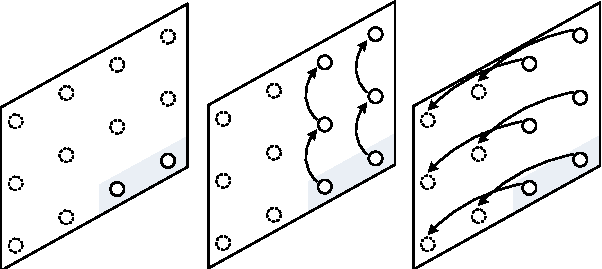
\includegraphics[width = 3in]{./FIGURES/fig5.pdf}
\caption {The window of currently available activations are extended vertically first and then horizontally.} \label{popgroup}
\end{figure} 
The number of the line delays added is
\begin{equation}
N_{linedelays} = (K_h-1)L_w.
\end{equation}
The number of the activation delays added is
\begin{equation}
N_{actdelays} = (K_w-1)(K_h+L_h-1).
\end{equation}
Then, the number of the total delays becomes
\begin{equation}
\begin{split}
N_{delays}& =  (W/L_w) N_{linedelays} + N_{actdelays}\\
 & = W(K_h-1) + (K_w-1)(K_h+L_h-1) .
\end{split}
\end{equation}
It is interesting to note that the number of the total delays does not depend on $L_w$.

\subsection{Extension for Stride, Arbitrary Input Size, and Borders}
It may be straightforward to unfold a given structure for parallel processing, but there are many non-trival issues in practical implementation of the parallel structure, especially for use in recent convolutional neural networks. For example, we may need a special handling for the case that $H$ ($W$) is not a multiple of $L_h$ ($L_w$).  In addition, we have assumed that the stride of the convolution is 1. 
However, non-one stride is commonly used for the first convolution layer and max-pooling in recent convolutional neural networks (CNNs). 
Besides, 2D filtering is cascaded in CNNs, and the size of the input maps changes from layer to layer.  
We extend the proposed method to deal with those practical issues. We will generate a parallel structure for a convolution with stride $S$. This convolution is a stage in cascaded filters.  For simplicity, we assume that $K \ge S$. We also suppose that $L$ is a multiple of $S$ if $L\ge S$ and $S$ is a multiple of $L$ otherwise. We will discuss the general case in the detail in the next subsection. When stride is not 1, the output block size becomes different from the input block size. Let $L_h' \times L_w'$ denote the output block size.
Considering stride, the size of a dimension of the group window becomes
\begin{equation}
	G = K + S(L'-1). 
\end{equation}
 
The 2D filter with stride $S$ downsamples by a factor of $S$, so we have   
\begin{equation}
%L' =  L/S.
L' = 
  \begin{cases}
    L/S       & \quad \text{if } L\ge S \\
    1         & \quad \text{if } L<S.\\
  \end{cases}
\end{equation}

We now extend the proposed method to handle the input of arbitrary size and the borders. For that, we introduce the \textit{bleed}, which is the area to be trimmed out.
We suppose that the input and the output of the parallel filter include the bleed. For the bleed, the values of the top $B$ rows and the left $B$ columns of the input map are meaningless. 
These values may be intentionally padded to make the input size a multiple of the block size, or may have been invalidated for a convolution in a previous stage. For the cascaded convolutions, we propagate the bleed without cropping it right away and it is trimmed out when $L'=1$ .

When we handle the border with cropping, the output bleed becomes
\begin{equation}
B' = (B + K-1) /S
\end{equation}
if $L'>1$. If $L'=1$, $B'=0$.
Since the border handling affects the bleed, not the size of the output, the size of the input maps change only due to stride. 
Since the output size is simply $W/S$ for the bleed, the output size becomes a multiple of $L'$. This means that if we make the input size for the first convolution a multiple of the block size by using the bleed, the alignment of the block is automatically taken care of in the subsequent convolutions.

We consider the group window of stride 1 even when we deal with non-one stride. We call it the \textit{pan-group window}. The group window is displaced by $mod(B+K-1,\min(S,L))$ to the right owing to the bleed and the border handling, and the group window is smaller than the pan-group window by $min(S,L)-1$. Thus, the right-bottom corner of the group window is away from that of the pan-group window by the margin
\begin{equation}
 	M = \min(S,L)-1-mod(B+K-1,\min(S,L))
\end{equation}
as shown in Figure~\ref{offset}.
\begin{figure}[h]
\centering
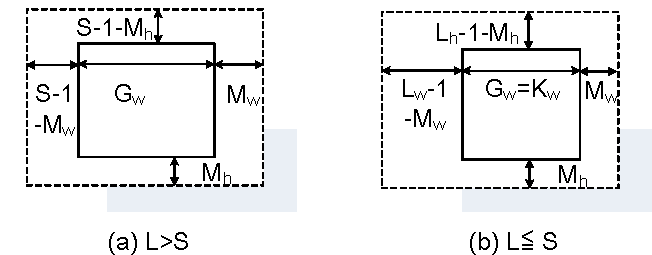
\includegraphics[width = 2.5in]{./FIGURES/fig6.pdf}
\caption {The dotted box indicates the par-group window. The group window is a smaller window within the par-group window.} \label{offset}
\end{figure} 


Some of the bleed may be replaced by zeros for zero padding and in order to pad zeros at the right and the bottom we can also decrease the left (top) bleed and increase the right (bottom) bleed by adding activation (line) delays. The time steps for the bottom bleed and some of the right bleed are borrowed from those for the next activation map.

 The overall algorithm is summarized in Algorithm~\ref{pgw}.  The size of the window of currently available activations is $L_h \times L_w$ initially (line 3). We extend this window vertically to the top using line delays until the height of the window becomes $G_h+M_h$ (line 4-6).  Then, we extend it horizontally to the left using activation delays until the width becomes $G_w+M_w$ (line 8-9). 

The number of the line delays added is
\begin{equation}
N_{linedelays} = (G_h+M_h-L_h)L_w.
\end{equation}
The number of the activation delays added is
\begin{equation}
N_{actdelays} = (G_w+M_w-L_w)G_h.
\end{equation}

Once the activations in the group window are available at the same time by the structure generated by the algorithm, each output is generated by using the activations in its kernel window. In neuromorphic architectures, each output is generated by a neuron connected to $K_hK_w$ synapses, so it requires $K_hK_wL_h'L_w'$ synapses and $L_h'L_w'$ neurons in total. For the remaining structure, the number of the resources required in conventional and neuromorphic implementations are summarized in Table~\ref{resource}. 

\begin{algorithm}\small                      % enter the algorithm environment
\caption{GenerateDelayStructure}          % give the algorithm a caption
\label{pgw}                           % and a label for \ref{} commands later in the document
\textbf{Input:} {$L_h \times L_w$ input nodes}
\begin{algorithmic}[1]                    % enter the algorithmic environment

\STATE Let $F$ be the two-dimensional array of nodes
\STATE Let $N_h$ and $N_w$ be the height and width of $F$
\STATE Initialize $N$ with $L_h\times L_w$ input nodes
\WHILE{$N_h<G_h+M_h$}
\STATE Expand $F$ vertically to the top by adding line delays 
\ENDWHILE
\WHILE{$N_w<G_w+M_w$}
\STATE Expand $F$ horizontally to the left by adding pixel delays for $G_h$ rows
\ENDWHILE
\STATE Remove $M_h$ rows in $N$ from the bottom
\RETURN $F$ 
\end{algorithmic}
\end{algorithm}

  \begin{figure*}
  \centering
  \begin{subfigure}{.22\textwidth}
    \centering
    \epsfig{figure = ./FIGURES/fig7a.pdf, width = \textwidth}
    \caption{}
  \end{subfigure}
  \begin{subfigure}{.22\textwidth} 
    \centering
    \epsfig{figure = ./FIGURES/fig7b.pdf, width = \textwidth}
    \caption{}
  \end{subfigure}
  \begin{subfigure}{.22\textwidth}
    \centering
    \epsfig{figure = ./FIGURES/fig7c.pdf, width = \textwidth}
    \caption{}
  \end{subfigure}
  \begin{subfigure}{.22\textwidth}
    \centering
    \epsfig{figure = ./FIGURES/fig7d.pdf, width = \textwidth}
    \caption{}
  \end{subfigure}
  \caption{Parallel filters improve the performance at the cost of circuit area. However, if stride is not one, it can improve the performance without any cost by increasing the utilization.  }\label{fdata}
  \end{figure*}
\begin{table}\small
	 \centering 
\caption{The number of the computational resources required depends on the output block size, not the input block size. }\label{resource}
\begin{tabular}{|c|c|c|c|}
\hline
Impl. Type   & Resource Type & Number of Resources   \\
   \hline
 
 & $N_{multipliers}$ & $K_h  K_w  L'_h  L'_w$\\
Conventional & $N_{adders}$ & $(K_h  K_w - 1 ) L'_h  L'_w$ \\
 & $N_{registers}$  & $K_h K_w$  \\
\hline
\multirow{2}{*}{Neuromorphic} & $N_{synapses}$ & $K_h  K_w  L'_h  L'_w$    \\
 & $N_{neuron}$  &   $L'_hL'_w $   \\ 
\hline
\end{tabular}\\\raggedright
\end{table}	

\subsection{Non-Integer Output Block Size}
If the block size is not a multiple of the stride, or the stride is not a multiple of the block size, we can increase the output block size by setting $L'=lcm(L, S)/S$ and decrease the sampling rate instead. However, in this case, the input size should also be a multiple of $lcm(L,S)$ for the output to be a multiple of $L'$.
If we encounter this case in a middle of the cascaded convolutions, and the input size is not such a multiple, then we can pad more bleed into the initial input, or remove some of the bleed in a previous stage. 

\section{Experimental Results}
  
  
We have implemented the proposed algorithm in Python. It takes a convolutional neural network and generates a time delay neural network (TDNN). We adopt the neuromorphic architecture proposed in~\cite{chung2015insight}. Each unit (connection) in the TDNN is implemented into a hardware neuron (synapse) based on a bit-serial adder (multiplier).  Each delay in the TDNN is also implemented in a hardware delay based on a shift-register. Then, there is an one-to-one mapping between the TDNN and the processing elements, and the TDNN is converted into a huge feedforward logic circuit described in Verilog where constants are hard-coded. The circuit is synthesized using Xilinx Vivado and is mapped into Xilinx Virtex 7 2000T FPGA. No DSP slice and block RAM are used.
  
  
First, we randomly generate a 2D filter with a 3$\times$3 kernel for a map of 32$\times$32 activations. 
In the neuromorphic architecture, there is no other performance bottleneck such as off-chip memory access and on-chip array access and the actual throughput increases as the block size increases as shown in Figure~\ref{fdata}(a).
Figure~\ref{fdata}(b) shows the number of delays when the block size (i.e., the level of parallel processing) varies. The block size has almost no impact on the number of delays, but depending the margin of the group window, the number of delays can even be reduced. Figure~\ref{fdata}(c) shows the number of synapses as the block size increases. As long as the stride is smaller than or equal to the block size, the number of synapses does not change. Thus, we can obtain almost free performance improvements until then. This is possible because the synapses are under-utilized when the block size is smaller than the stride. 
Figure~\ref{fdata}(d) shows the synthesis results of the filters with different block sizes. The figure is very well correlated with Figure~\ref{fdata}(c) because the synapses occupy most area of the circuit.

\begin{table}\scriptsize
	 \centering 
\caption{When the $1\times 1$ block size meets stride $S>1$, the utilization decreases 1/$S^2$. }\label{case1}
\begin{tabular}{|c|c|c|c|c|c|c|c
	c|}
\hline
\multirow{3}{*}{Layer Type }&  \multicolumn{2}{c|}{Min-Area Design~\cite{chung2015insight}}  &  \multicolumn{4}{c|}{$2\times2$-Parallel Design}  \\
\cline{2-7}
   & Input & \multirow{2}{*}{Utilization}  & Block  & Input &  \multirow{2}{*}{Util.} &\multirow{2}{*}{Bleed}    \\
   & Size  &       & Size   & Size &  &\\
   \hline

3$\times$3 conv~~~ & 32 & 1 & 2$\times$2 & 32 & 1 & 0 \\
3$\times$3 conv~~~ & 30 & 1 & 2$\times$2 & 32 & 1& 2\\
4$\times$4 pool-s2 & 28 & 1 & 2$\times$2 & 32 & 1 & 4\\
3$\times$3 conv~~~ & 13 & 0.25 & 1$\times$1 & 13 & 1 &0  \\
3$\times$3 conv-p1 & 11 & 0.25  & 1$\times$1 &  11 & 1 &0\\
4$\times$4 pool-s2 & 11 & 0.25  & 1$\times$1 & 11 & 1 &0\\
fc &  4 & 0.0625 & 1$\times$1 &  4 & 0.25 &0    \\
fc &  1 & 0.0625 & 1$\times$1 &  1 & 0.25 &0 \\

\hline
\end{tabular}\\\raggedright
\end{table}	

\begin{table*}\scriptsize
\centering

\caption{A time delay neural network is converted into a logic circuit and it is implemented in two different flavors. The convolutional layers of AlexNet are executed at unprecedented energy-efficiency.}\label{final_table}
\begin{tabular} {|c|c|c|c|c|c|c|c|c|c|c|c|c|c|c|c|c|}
\hline

\multirow{3}{*}{Datasets} & \multirow{2}{*}{Block} & \multicolumn{5}{c|}{TDNN Model} &     \multicolumn{5}{c|}{Maximum Performance Design} & \multicolumn{5}{c|}{Minimum Power Design} \\
\cline{3-7}
\cline{8-17}
&  \multirow{2}{*}{Size} & \multicolumn{3}{c|}{Delay}    & \multirow{2}{*}{Neuron}&\multirow{2}{*}{Synapse} &Area &Images &\multicolumn{3}{c|}{Power (W)} &Area &Images &\multicolumn{3}{c|}{Power (W)} \\
\cline{3-5}
\cline{10-12}
\cline{15-17}
& & Line & Act.&Total&&&(LUTs)&/sec&Dyna.&Static&Total&(LUTs)&/sec &Dyna. &Static&Total\\
\hline

\multirow{2}{*}{CIFAR}& 1$\times$1 &  846 & 4366 & 18973   & 4091 & 16151 & 109169 &4882 & 1.4 &0.668&2.068 & 109169 & 4882 & 1.4 &0.668&2.068\\
\multirow{2}{*}{10}& 1$\times$2 &     1080 & 4114 & 18721    & 5412 & 19443 & 131899  &9764 & 2.4 &0.689&3.089 & 135112 & 4882 & 1.2 &0.661&1.861\\
 & 2$\times$2 &     954 & 4160 & 16751    & 8052 & 26027 & 169462  &19528 & 3.4 &0.707&4.107 & 169759 & 4882 & 0.6 &0.653&1.253\\
\hline
 & 1$\times$1  & 2207 & 29221 & 87678 &17470 & 90110 & 495232 &97 &4.4 & 1.007 & 5.407 &495232&97&4.4&1.007&5.407\\ 
ILVSRC & 1$\times$2 & 2237 & 23531& 82018 &17688 &90118 &496217 &194 &4.4 & 1.003 &5.403 &496098 &97&2.2&0.791 &2.991\\
2012 & 2$\times$2 & 2231 & 23531 & 81334 &17694& 90134  & 494769 &388 &5 & 1.008 &6.008 &494704 &97&1&0.713 &1.713\\
  & 4$\times$4 & 2261 & 23465 & 79900 &17606& 90230 & 494777 &776 &6.2 & 1.021 &7.221 &494630 &97 &0.2 &0.663 &0.863\\

\hline
\end{tabular}
\end{table*}



\begin{figure}
\centering
\begin{subfigure}{.22\textwidth}
  \centering
  \epsfig{figure = ./FIGURES/fig8a.pdf, width = \textwidth}
  \caption{}
	\end{subfigure}
\begin{subfigure}{.22\textwidth}
  \centering
  \epsfig{figure = ./FIGURES/fig8b.pdf, width = \textwidth}
  \caption{}
\end{subfigure} 
\caption{The energy-efficiency increases as the block size increases. The high-frequency designs show higher efficiency since lowing the operating frequency scales the dynamic power only.  }\label{cifar}
\end{figure}

Next, we use the 6-layer convolutional neural network described in Table~\ref{case1} for the CIFAR-10 task. This network achieves 84.43\% classification accuracy and is simplified to a sparse network with 18K parameters using the method of~\cite{chung2016simplifying} and the accuracy becomes 80.96\%. After quantizing the weights to 5 bits, it becomes 80.61\%. Then, we convert the convolutional layers into the activation-serial (baseline) and the proposed activation-parallel structures varying the block size and the whole network turns into a TDNN.
Table~\ref{case1} shows two different designs for the 6-layer convolutional neural network and the min-area, baseline design is the one proposed in~\cite{chung2015insight}. In the layer type, `s' stands for stride and `p' means zero padding. All the layers have stride 1 and no zero padding unless otherwise stated. In the min-area design, the hardware utilization decreases 1/$S^2$ for stride $S$. Considering that, if we set the block size of the first layer to the sum of the non-one strides in the net, we can even make a full-utilization design. In the pixel-parallel design, the input for each layer includes the bleed and the input size does not change due to the border handling. The block size, the input size and the bleed decrease when non-one stride is encountered as in the third layer. When the output block size becomes one, the bleed is trimmed out. 

 Table~\ref{final_table} shows the statistics of the TDNNs and the FPGA implementation results. For the 1$\times$2 design, the number of the line delays increase, but the number of delays in a line delay decreases in the parallel structures. As the block size increases, the total number of delays decreases and it can happen when we generate the parallel structures for non-one stride. The dynamic power is measured at 220V AC and the efficiency of the AC-DC conversion is around 70\%. All the dynamic power measurements include the inefficiency of on-board regulators as well. The static power is obtained from the power reports of Vivado. When the block size increases, we can increase the throughput by running the designs at the same frequency (Max. Performance Designs). Or, we can reduce the power consumption while maintaining the performance by decreasing the clock frequency. (Min. Power Designs). The baseline design is under-utilized because of pooling as shown in Table~\ref{case1} and increasing the block size improves the utilization, and hence the energy-efficiency. As the block size increases, the number of LUTs increases slowly because only the layers earlier than the first pooling are parallelized. Figure~\ref{cifar} shows the energy-efficiency of the CIFAR-10 designs.


 To validate the proposed method further, we use the convolutional layers of AlexNet~\cite{krizhevsky2012imagenet} for the ImageNet large-scale natural image classification task. We use AlexNet without the local response normalization layers, and the baseline model achieves 52.46\% top-1 accuracy. To use this network in a neuromorphic architecture, we simplify the convolutional layers until it has 100K parameters and the accuracy becomes 50.36\%. After quantizing the weights to 5 bits, the accuracy becomes 49.23\%. Table~\ref{final_table} shows the implementation results for various block sizes. In AlexNet, the first convolutional layer has stride of 4 and we can increase the performance or decrease the power consumption with almost no area penalty, achieving unprecedented energy efficiency using off-the-shelf FPGAs.

\section{Conclusion}
We have proposed the methods to synthesize parallel structures for the convolutional layers of recent convolutional neural networks. We have dealt with practical issues such as border handling and alignment by introducing the bleed. The neuromorphic computing system based on activation-serial structures already demonstrated high energy-efficiency and performance, but the activation-parallel structures have allowed us to show that the nearly bottleneck-free architecture can have unparalleled efficiency and performance.    

\ifCLASSOPTIONcaptionsoff
  \newpage
\fi

\bibliographystyle{unsrt} 
\bibliography{scibib}

\end{document}



